%% -*- TeX-master: t -*-

\documentclass[draft]{acm_proc_article-sp}

\newcommand{\thetitle}[0]{Statistical Debugging Using Compound Boolean Predicates}
\newcommand{\wraptitle}[0]{Statistical Debugging Using \\ Compound Boolean Predicates}

\pagenumbering{arabic}

%%%%%%%%%%%%%%%%%%%%%%%%%%%%%%%%%%%%%%%%%%%%%%%%%%%%%%%%%%%%%%%%%%%%%%%%
%%
%% standard texmf packages
%%

% font selection
\usepackage[T1]{fontenc}
\usepackage{courier}
\usepackage[scaled]{helvet}
\usepackage{mathptmx}

\usepackage{booktabs}
\usepackage{flushend}
\usepackage[final]{graphicx}
\usepackage{hyphenat}
\usepackage{nicefrac}
\usepackage{paralist}
\usepackage[dvips]{thumbpdf}
\usepackage{xspace}

\usepackage[
bookmarks,
breaklinks,
draft=false,
pdftitle={\thetitle},
pdfauthor={Piramanayagam Arumuga Nainar, Ting Chen, Jake Rosin, and Ben Liblit},
% pdfsubject={D.2.4 [Software Engineering]: Software/Program Verification -- statistical methods; D.2.5 [Software Engineering]: Testing and Debugging -- debugging aids, distributed debugging, monitors, tracing; I.5.2 [Pattern Recognition]: Design Methodology -- feature evaluation and selection},
% pdfkeywords={bug isolation, random sampling, invariants, feature selection, statistical debugging},
]{hyperref}

%% \VerbatimFootnotes

%%%%%%%%%%%%%%%%%%%%%%%%%%%%%%%%%%%%%%%%%%%%%%%%%%%%%%%%%%%%%%%%%%%%%%%%
%%
%% unique to this report
%%

\newdef{defn}{Definition}
\newcommand{\defnautorefname}[0]{Definition}

\newcommand{\Importance}[0]{\mathit{Importance}\xspace}
\newcommand{\Increase}[0]{\mathit{Increase}\xspace}
\newcommand{\NumF}[0]{\mathit{Increase}\xspace}
\newcommand{\effort}[0]{\mathit{effort}\xspace}

\newcommand{\obs}[2]{#1(\text{$#2$ observed})}

\newcommand{\true}[0]{\mathit{true}\xspace}
\newcommand{\false}[0]{\mathit{false}\xspace}
\newcommand{\unknown}[0]{\mathit{unknown}\xspace}

\newcommand{\prog}[1]{\texttt{#1}}
\newcommand{\func}[1]{\texttt{#1}}

\renewcommand{\sectionautorefname}[0]{Section}
\renewcommand{\subsectionautorefname}[0]{\sectionautorefname}
\renewcommand{\subsubsectionautorefname}[0]{\sectionautorefname}


%%%%%%%%%%%%%%%%%%%%%%%%%%%%%%%%%%%%%%%%%%%%%%%%%%%%%%%%%%%%%%%%%%%%%%%%
%%
%% front matter
%%

\title{\wraptitle}

\newcommand{\mailto}[1]{\href{mailto:#1@cs.wisc.edu}{#1}}

\numberofauthors{1}
\author{\alignauthor
  Piramanayagam Arumuga Nainar \qquad Ting Chen \qquad Jake Rosin \qquad Ben Liblit \\
  \affaddr{Computer Sciences Department} \\
  \affaddr{University of Wisconsin--Madison} \\
  \email{\{\mailto{arumuga},\mailto{tchen},\mailto{rosin},\mailto{liblit}\}@cs.wisc.edu}}

%%%%%%%%%%%%%%%%%%%%%%%%%%%%%%%%%%%%%%%%%%%%%%%%%%%%%%%%%%%%%%%%%%%%%%%%
%%
%%  document body
%%


\begin{document}

\maketitle

\begin{abstract}
Cooperative Bug Isolation (CBI) is a technique to find bugs in programs that analyzes data collected from program executions.  At each program point, CBI identifies boolean expressions, called as predicates, to be instrumented.  We augment CBI's bug predictive ability by combining these predicates using logical operators (conjunction and disjunction).  The motivation is that a complex predicate will provide more information to the programmer by narrowing down possible program states.  Our experimental results show that the scores of complex predicates are usually higher or atleast comparable to single predicates.  This makes them good indicators of bugs.  We discuss a new metric that uses program structure to quantify the usefulness of complex predicates.  Using this metric, we could eliminate a large number of spurious predicates from consideration.  Finally we discuss the effect of sparse random sampling on the usefulness of complex predicates.

\end{abstract}
% -*- TeX-master: "report" -*-

\section{Introduction}

Statistical debugging improves software quality by identifying program (mis)behaviors that are highly predictive of subsequent program failure.  As embodied in the Cooperative Bug Isolation Project (\emph{CBI}) \cite{Liblit:2004:CBI}, these techniques find bugs in programs by analyzing reports collected from software executing in the hands of end users.  First the CBI instrumenting compiler injects extra code that evaluates simple Boolean expressions (called \emph{predicates}) at various program points.  Predicates are designed to capture potentially interesting program behaviors such as results of function calls, directions of branches, or values of variables.  Upon termination of an instrumented program, a feedback report is generated that records how often each predicate was observed, and how often each was both observed and found to be true.  Given many such feedback reports, e.g., from a large user community, statistical debugging is used to find predicates that are predictive of failure \cite{Liblit:2005:SSBI,Zheng:2006:SDSIMB}.  These predicates are then ranked and presented to the developer.

CBI gathers execution reports by using valuable CPU cycles at end user machines.  It is essential to make those cycles worthwhile by extracting every bit of useful information from them.  However, current statistical analysis algorithms consider predicates in isolation from one another \cite{Liblit:2005:SSBI,Zheng:2006:SDSIMB}.  They overlook potentially useful relations between predicates.  Predicates are expressions involving program variables at different program points and hence may be related by control and data dependences.  We propose to capture these relations by building \emph{complex predicates} from the set of currently instrumented predicates (which we refer to as \emph{simple predicates}).  Since predicates are Boolean expressions, they are combined using logical operators (such as conjunction and disjunction).  We construct complex predicates and include them in the input to the statistical analysis algorithms.

There are two approaches to combine predicates using logical operators:
\begin{enumerate}
\item Change the instrumenting compiler to explicitly monitor each complex predicate at run time.
\item Estimate the value of each complex predicate from the values of its components.
\end{enumerate}

The first approach will yield a precise value but needs significant modifications to existing infrastructure.  The second approach will be less precise (as described later) but requires only few modifications to existing infrastructure (and none to the instrumenting compiler).  In the present work, we implement the second approach, which serves as a proof of concept for using complex predicates, as well as a justification for a future attempt at incorporating them into the compiler.

The remainder of this paper is organized as follows.  \autoref{sec-bground} reviews statistical debugging and motivates the present effort to find complex failure predictors.  \autoref{sec-complex-preds} gives a precise definition of complex predicates and discusses the trade-offs in our implementation.  \autoref{sec-metrics} defines two metrics to evaluate the usefulness of a complex predicate.  \autoref{sec-qual} discusses two case studies that demonstrate the usefulness of complex predicates.

\autoref{sec-experiments} presents the results of experiments conducted on a large suite of buggy test programs, including an assessment of the effect of sparse random sampling on complex predicates.  Sparse random sampling is a technique used by CBI to reduce the runtime overhead of instrumentation.  \autoref{sec-rw} discusses related work and \autoref{sec-conc} concludes.

% -*- TeX-master: "report" -*-

\section{Background}
\label{sec-bground}
CBI uses lightweight instrumentation to collect feedback reports that contain truth values of predicates in an execution as well as the outcome{\footnote{crash and non-crash or some other binary classification}} of the execution.  A large number of these reports are collected and analyzed using statistical debugging techniques.  The analysis described in~\cite{Liblit:2005:SSBI} computes a numeric score corresponding to each predicate.  The score is called $\Importance$ and is computed as follows:

The truth values of a predicate $P$ from all the runs can be aggregated into four values:

\begin{enumerate}
\item $S$($P$ observed) and $F$($P$ observed), the number of successful and failed runs respectively, in which the value of $P$ was evaluated.
\item $S$($P$) and $F$($P$), the number of successful and failed runs respectively, in which the value of $P$ was evaluated and was found to be true.
\end{enumerate}

Using these values, two scores of bug relevance are calculated.  They are:
\begin{enumerate}
\item $F$($P$).  A good predictor must predict a large number of failed runs.
\item $\Increase(P)$, the amount by which $P$ being true increases the probability of failure over simply reaching the line where P is defined.  It is computed as follows:

\begin{equation}
\label{eqn1}
\Increase(P) \equiv
\frac{F(P)}{S(P) + F(P)}
-
\frac{F(\text{$P$ observed})}{S(\text{$P$ observed}) +
  F(\text{$P$ observed})}
\end{equation}
\end{enumerate}

Both of these scores are independent but good dimensions of a bug predictor.  These dimensions are combined into a single value by taking their harmonic mean.  Since $\Increase(P)$ is bounded by 1, the $F(P)$ component in $\Importance$ is normalized over the total number of failed runs $\NumF$ after a logarithmic transformation.  The overall metric is:
\begin{equation}
\label{eqn2}
\Importance(P) \equiv
\frac{2}{
  \frac{1}{\Increase(P)}
  +
  \frac{1}{log(F(P)) / log(\NumF)}}
\end{equation}

To eliminate different predicates that predict the same bug, only the top ranked predictor is presented to the user.  To handle the case where multiple bugs are present, all the failed runs in which the top predicate is true are eliminated and the remaining predicates are ranked by recomputing their scores in the remaining set of runs.  This process of eliminating runs continues until there are no remaining failed runs or no remaining predicates.

The output of the analysis will contain the list of predicates that had the highest score during any iteration of the redundancy elimination algorithm.  This list can be used by the programmer to track down bugs, or as input to other automated analysis tools.

\subsection{Expected Benefits}

Complex predicates can improve the analysis described above in three ways:
\begin{inparaenum}[(1)]
  \item provide a richer diagnostic language for complex bugs,
  \item better recall and precision for both complex and simple bugs, and
  \item enhanced support of automated tools that further process CBI output.
  \end{inparaenum}

\paragraph{Richer Diagnostic Language for Complex Bugs}

A single predicate can be thought of as partitioning the space of all runs into two subspaces: those satisfying the predicate and those not. Bugs with easily-described causes partition cleanly using a single bug predictor, with (all or most) successes in one subspace and (all or most) failures in the other.  If a bug has a simple cause, and this cause corresponds well to a simple predicate, then a simple analysis is sufficient.

However, the success/failure boundary may be considerably more irregular.  A richer language of candidate bug predictors describes more complex shapes within the space of runs, and thereby diagnoses the causes of more complex failures.  Of course, a fiendishly convoluted (but hopefully rare) bug may require a predicate as complex as the entire original program to describe its behavior.  Thus, there is a balance to be struck: the language of complex predicates should be expressive enough to describe important bugs, but not so expressive as to become unwieldy in practice.  The present research explores one possible point on this complexity spectrum.

\paragraph{Improved Precision and Recall}

We hypothesize that complex predicates will be especially helpful in coping with \emph{super-} and \emph{sub-bug predictors}, a challenging aspect of statistical debugging first identified by Liblit et al. \cite{Liblit:2005:SSBI}.

A \emph{super-bug predictor} is one that is true in a large number of failures but also true in a large number of successful runs.  In other words, it is not a specific enough predictor of failure.  In information-retrieval terms, a super-bug predictor has high recall but low precision.  A possible (but not the only) cause for super-bug predictors is a non-deterministic bug that does not necessarily cause a failure when it is triggered.  In the most extreme case, a super-bug predictor may be complete (predicts all failures) but not sound (predicts some successes also).  False positives could be reduced or eliminated by taking a conjunction of this predictor with another predicate that captures another aspect of the bug.

A \emph{sub-bug predictor} is one that is true in a small number of failed executions.  In other words, it is not sensitive enough to predict all instances this failure.  In information-retrieval terms, a sub-bug predictor has high precision but low recall.  In the most extreme case, a sub-bug predictor may be sound (predicts only failures) but not complete (does not predict all failures).  False negatives could be reduced or eliminated by taking a disjunction with another predictor can captures other instances of the bug.  It is important to note that in software with multiple bugs, the analysis may find a disjunction of predictors of individual bugs as a predictor for the whole set of failures.  The user should keep this in mind while using a disjunction predictor to track down a bug.

A \emph{perfect bug predictor} is one that is true in all failed executions and false in all successful ones: in other words, it is both sound and complete.  Such predictors indicate a bug which is completely deterministic given the involved predicates.  Generally speaking, the closer a predictor is to perfect the more informative it is to a programmer.  By eliminating false positives and negatives conjunctions and disjunctions can move super- and sub-bug predictors closer to perfection.

\paragraph{Enhanced Support of Automated Tools}

Bug predictors identified by statistical debugging can be useful to humans directly, or can serve as input to other automated tools and analyses.  In the later case, it may be feasible to use even richer, more complex, or more numerous predictors that a human would find overwhelming if examined directly.  \textsc{BTrace}~\cite{Lal:2006:POPAD} is one such tool. \textsc{BTrace} finds the shortest control- and dataflow-feasible path in the program that visits a given set of bug predictors.  More predictors, and predictors drawn from a more expressive language, can better guide \textsc{BTrace}'s path exploration toward paths which accurately reflect the sequence of events leading to failure.

\section{Complex Predicates}
\label{sec-complex-preds}
This section gives a precise definition of complex predicates and discusses the trade-offs in our implementation.

A complex predicate $C$ is defined as $C = \phi(p_1, p_2, \ldots p_k)$ where $p_1, p_2, \ldots p_k$ are simple predicates and $\phi$ is a function that can be computed using only the logical operators $and$ and $or$.  The operator $not$ is not required because any propositional formula can be written in conjunctive normal form (CNF) in which the $not$ operator appears only before the literals.  And by design, the negation of every simple predicate $P$ is also a predicate.

For a predicate $P$ and a run $R$, $R(P)$ is true if $P$ was observed to be true atleast once during run $R$.  Similarly we could define $R(C)$ as follows:
\begin{defn}
\label{dfn1}
For a complex predicate $C = \phi(p_1, p_2, \ldots p_k)$, $R(C)$ = 1 iff at some point during the execution of the program, $C$ was observed to be true.
\end{defn}

The difficulty with this notion of the complex predicate is that $C$ must be explicitly monitored during the program execution.  For example, if $C_1 = p_1 \wedge p_2$ then $R(p_1)$ = 1 and $R(p_2)$ = 1 does not imply that $R(C)$ = 1.  $p_1$ and $p_2$ may be true at different stages of execution but never true at the same time.  However, as discussed earlier, explicitly monitoring $C$ requires significant changes to existing infrastructure.  In order to be able to estimate the value of $C$ from its components, we adapt a less precise definition as follows:
\begin{defn}
\label{dfn2}
For a complex predicate $C = \phi(p_1, p_2, \ldots p_k)$, $R(C)$ = 1 iff $\phi(R(p_1), R(p_2), \ldots R(p_k))$ = $true$
\end{defn}

In other words, we consider that $R$ as distributive over $\phi$.  This can lead to false positives, because $R(C)$ may be computed to 1 when it is actually 0, but no false negatives.  The impact of this assumption on the score of $C$ may be either positive or negative depending on whether $R$ failed or succeeded.

There are $2^{2^N}$ boolean functions of $N$ predicates ~\cite{MathWorld:BoolFuncs}.  This is a prohibitively large number considering that there can be hundreds of simple predicates.  To reduce the complexity, we consider only functions of two predicates.  There are $2^{2^2}$ = 16 such functions and their arguments can be chosen from $N$ predicates in $^NC_2 = \frac{N(N-1)}{2}$ ways.  Out of the 16 boolean functions of two variables, we restrict only to conjunction ($and$) and disjunction ($or$) since other functions are more complex and cannot be used effectively by the programmer.  Other functions can be easily included in our implementation once their truth table (discussed later) are derived correctly.  Thus, we evaluate only $2. ^NC_2 = N(N-1)$ functions for building complex predicates.  If $R$ is the set of runs being analysed then the time complexity required to build complex predicates is $|R|N(N-1) = O(|R|N^2)$

Even after imposing many constraints, the number of complex predicates is quadratic in the number of simple predicates.  A large number of complex predicates formed by this procedure are likely to be useless in the analysis of the program.  A complex predicate that has a lower score than its components is useless.  The component (simple) predicate with a higher score is a better predictor of failure, and so the complex predicate adds nothing to the analysis.

\begin{defn}
\label{dfn3}
A complex predicate $C = \phi(p_1, p_2, \ldots p_k)$ is ``interesting'' if $Importance(C) > Importance(p_i)$ for $i \in \{1, 2, \ldots k\}$
\end{defn}

In the case where the complex predicate has the same score as the component predictor with higher score, the simpler one is preferable.  Definition ~\ref{dfn3} is for the general case and as explained earlier, we explore only for $k = 2$ and $\phi \in \{\vee, \wedge\}$.  Keeping only interesting combinations of predicates reduces the memory burden of storing them, and helps ensure the utility of a complex predicate that passes inspection.

\subsection{Pruning}
Forming a complex predicate from two components is a nontrivial task, requiring a conjunction or disjunction for each program run.  After this computation is complete the score of the newly formed predicate can be calculated, potentially labeling it uninteresting.  In such a case the effort to form the predicate has been wasted.  This provides the motivation to prune combinations early based on an estimate of their resulting scores.  An upper bound for a predicate's score can be determined by maximizing $F(P)$ and $Increase$ under constraints based on the propositional operation.  The score of the predicate, being a harmonic mean of these two terms, will likewise be maximized.

--figure of Increase--

--subsection: pruning disjunctions--

--figure of the terms for a disjunction--

Disjunction in this context can be considered the union of the set where $P1$ and that where $P2$.  The size of the resulting set is maximized when the two do not overlap, and that is the assumption made when calculating an upper bound on $F(P)$.  $S(P)$ is minimized by making the opposite assumption - that one is a subset of the other.  The size of the union is thus the size of the superset.

The second term in $Increase$ can only reduce the result, and so it is ignored in calculating an upper bound.

--subsection: pruning conjunctions--

--figure of the terms for a conjunction--

Conjunction can be regarded as set intersection.  Maximizing $F(P)$ requires that one of the intersecting sets is a subset of the other, making the size of the intersection the size of the smaller operand.  A minimal $S(P)$ is found when the component sets are nonoverlapping; the union of two such sets is empty.

If the second term is ignored, as with disjunctions, the upper bound of a conjoined predicate's $Increase$ score is 1.  This is the maximum $Increase$ possible, reducing the likelihood of a conjoined predicate being pruned to almost zero.  The second term is therefore used for conjunctions to drop the upper bound to a more useful level.

$F(P Observed)$ is minimized by assuming that $P$ was observed only in the (failed) runs where it was true.  Maximizing $S(P Observed)$ is more difficult.  Recall that a conjunction can be considered \textit{Observed} if either component is \textit{Observed False}, or both are \textit{Observed True}.  The intersection of successful runs where a predicate is \textit{Observed False} is maximized if the sets are nonoverlapping, while the intersection where they are \textit{Observed True} is maximized if one is a subset of the other.  By assuming both cases meet that criteria $S(P Observed)$ can be maximized.  Its value is the sum of successful runs where $P1 Observed$ and those where $P2 Observed False$, formed as the difference between $S(P2 Observed)$ and $S(P2)$.  Since the result may differ depending on which predicate is chosen as $P1$ the larger result is used.


% -*- TeX-master: "master" -*-

\section{Effort Metric}
\label{sec-metrics}
In our experiments, we often observe hundreds of complex predicates with similar or even identical high scores.  The redundancy elimination algorithm will select the top predicate randomly from all those tied for the top score; a human programmer finding a predicate to use in debugging is likely to make a similar choice.  Since $\Importance$ measures predictive power all high-scoring predicates should be good bug predictors, but even a perfect predictor may be difficult for a programmer to use in finding and fixing a bug.

Bug-fixing using a simple predicate is aided by understanding the connection between the predicate and the bug it predicts; for a complex predicate, the programmer must also understand the connection between its components.  Given a set of complex predicates with similar high scores, those that can be easily understood by a human are preferable.  In this section we propose two metrics based on this criteria for selecting predicates from the large set of highly-scored predictors.  Only predicates selected by the metrics are presented to the user (if predicate data is to analyzed by an automated tool it may not be advantageous to employ these metrics).  Both metrics use criteria unrelated to a predicate's $\Importance$ score, making them orthogonal to pruning as discussed in \autoref{sec-pruning}.

The first metric models the debugging effort required from the programmer to find a direct connection between component predicates.  We adapt the distance metric of Cleve and Zeller \cite{1062522} for this purpose.  In this metric, the score of a predicate is the fraction of code that can be ignored while searching for the bug.  We use a similar metric called \emph{effort} for a complex predicate.

\begin{defn}
\label{def-effort}
The effort required by a programmer while using a complex predicate $\phi(p_1, p_2)$ is inversely proportional to the smaller fraction of code ignored in a breadth-first bidirectional search for $p_1$ from $p_2$ and vice-versa.
\end{defn}

The idea behind this metric is that the larger the distance between the two predicates, the greater the effort required to understand their relationship.  Also, if a large number of other branches are seen during the search, the programmer should keep track of these dependencies too.  Per Cleve and Zeller \cite{1062522}, we use the program dependence graph (PDG) to model the program rather than the source code. We perform a breadth-first search starting from $p_1$ until $p_2$ is reached and count the total number of vertices visited during the search. The fraction of code covered is the ratio of the number of visited vertices to the total number of PDG vertices. 

The second metric is to consider the correlation between the two predicates.  Two predicates may be easily reached from one another without having an apparent connection - a complex predicate formed from them would provide little help to the programmer.  On the other hand, two predicates which are both affected by some shared area of code may have a connection which a programmer can easily discern.  The correlation between two predicates is defined based on the program dependency graph.  Given a single predicate $p$, we define its \textit{predecessor set} as the set of vertices in the PDG that can influence $p$.

\begin{defn}
\label{dfn5}
The correlation between two predicates of a complex predicate is defined as the number of vertices in the intersection of the two predecessor sets.
\end{defn}

The idea behind this metric is that a larger intersection between the $predecessor\ sets$ means it is possible that they are closely related.  We expect correlation to mitigate the issue of disjunctive predicates raised in \autoref{sec-background}, namely that the disjunction of predictors for two separate bugs will be scored very highly.  The predictors of two unrelated program faults are likely to reside in different areas of the program, and therefore the intersection of their predecessor sets would be smaller than two related predictors for the same bug, which are likely to be in closer proximity.

%Changed ``higher'' to ``better'' in the second-to-last sentence below, since what we actually want for metric 1 is a *lower* result.
The above two metrics could be applied both \emph{proactively} and \emph{reactively}.  A proactive use of the metrics will remove complex predicates whose metric values fall below a certain threshold of usefulness.  This will eliminate them from being computed and hence improve performance.  A reactive use of the metrics will retain all the predicates but break ties by giving higher ranks to those with better values for the metrics. This is desirable if neither computing time nor space is a concern.  We use CodeSurfer to build the PDG of a program and to compute these two metrics.


\section{Case Studies}
\label{sec-qual}
This section discusses two cases where complex predicates prove to be useful.  The first study is about a memory access bug in Exif 0.6.9, an open source image manipulation program.  A complex predicate was useful in increasing the score of an extremely useful bug predictor.  The second study uses an input validation bug in Ccrypt 1.2 to explain how complex predicates can be used to detect $super$ bug predictors automatically.

\subsection{Exif}
Exif 0.6.9 crashes while manipulating a thumbnail in a Canon image.  The bug is in function \texttt{exif\_mnote\_data\_canon\_load} in the module handling Canon images.  The following is a snippet from said function:
\begin{quote}
\begin{verbatim}
for (i = 0; i < c; i++) {
    ...
    n->count = i + 1;
    ...
    if (o + s > buf_size) return;    (a)
    ...
    n->entries[i].data = malloc(s);  (b)
    ...
}
\end{verbatim}
\end{quote}

The function skips the call to \texttt{malloc} that allocates memory to the pointer \texttt{n->entries[i].data} when \texttt{o + s > buf\_size}.  The program crashes when another function \texttt{exif\_\-mnote\_\-canon\_save} reads from \texttt{n->entries[i].data} without checking if the pointer is valid.  This is an example of a non-deterministic bug as the program succeeds as long as the uninitialized pointer is not accesed somewhere else.

We generated 1000 runs of the program using randomly generated command line arguments and input images randomly selected from a set of Canon and non-Canon images.  There were 934 successful executions and 66 crashes.  Applying the redundancy elimination algorithm with only simple predicates produced two predicates that account for all failed runs as shown in ~\autoref{tab:tbl1}.  Studying the source code of the program did not show any obvious relation between the two predictors and the cause of failure.  Even though the second predicate is present in the crashing function it was a comparison between two unrelated variables: the loop iterator \texttt{i} and the size of the data stored in the traversed array \texttt{s}.  Also it was $true$ in only 31 of the 66 failures.

\begin{table*}
\nocaptionrule
\caption{Results for Exif with only simple predicates}
\label{tab:tbl1}
\centering
\scriptsize
\begin{tabular}{lllll}
\toprule
initial & effective & Predicate & Function & File:line \\
\midrule
0.704974 & 0.704974 & new value of len == old value of len & jpeg\_data\_load\_data() & exif-0.6.9/libjpeg/jpeg-data.c:224 \\
0.395001 & 0.589484 & i == s & exif\_mnote\_data\_canon\_save() & libexif-0.6.10/libexif/canon/exif-mnote-data-canon.c:176 \\
\bottomrule
\end{tabular}
\end{table*}

The analysis had assigned a very low score of 0.0191528 to the predicate $P$: \texttt{o + s > buf\_size} despite the fact that it captures the exact source of the uninitialized pointer.  Because the bug was non-deterministic, $P$ was also $true$ in 335 runs that succeeded.  Including complex predicates in the analysis resulted produced one complex predicate shown in ~\autoref{tab:tbl2}{\footnote{the second row is the second component of a complex predicate, which is a conjunction as indicated by the keyword $and$ at the start}}.  Conjunction of $P$ with the second predicate $P'$: \texttt{offset < len} eliminated all the false positives and thereby assigning a very high score.  This is an example of how a conjunction can improve the score of a $super$ bug predictor.  $P'$ is in function \texttt{exif\_data\_load\_data} that calls exif\_mnote\_data\_canon\_load indirectly.  It is possible that it captures another condition that drives the bug to cause a crash.  If it does, it has to be a deep relationship as we could not find such a relation even after spending a couple of hours trying to understand the source.  However this does not reduce the importance of this result as the conjunction has a very high score compared to $P$ and $P'$.

\begin{table*}
\nocaptionrule
\caption{Results for Exif with complex predicates}
\label{tab:tbl2}
\centering
\scriptsize
\begin{tabular}{lllll}
\toprule
initial & effective & Predicate & Function & File:line \\
\midrule
0.941385 & 0.941385 & o + s $>$ buf\_size is TRUE & exif\_mnote\_data\_canon\_load &
 libexif-0.6.10/libexif/canon/exif-mnote-data-canon.c:237 \\
 
         &          & $and$ offset $<$ len & exif\_data\_load\_data & libexif-0.6.10/libexif/exif-data.c:644 \\
\bottomrule
\end{tabular}
\end{table*}

A good predictor that could be found using a CBI style analysis is $Q$: \texttt{n->entries[i].data == 0} or some predicate equivalent to it.  Scanning the source file shows that there is no such predicate that is currently instrumented by CBI.  If a future instrumentation scheme{\footnote{one suggestion is a predicate on scalar parameters to function calls}} instruments $Q$, then even an analysis with simple predicates will find $Q$ as the top bug predictor.  However, $P$ is still more useful than $Q$ in identifying the actual source of the $null$ pointer.  In fact, $P \wedge Q$ will be the perfect result as it captures the bug (skipping the \texttt{malloc}) and the trigger (the point where the illegal memory access is performed).  Thus, this bug in Exif presents a compelling evidence that complex predicates can be better bug predictors.

\vspace{4pt} \noindent
% If there are threats in other places, put this in a separate section
{\bf Threats to validity:}  There are some internal threats to the validity of the above experiment.  Firstly, Exif 0.6.9 had two other bugs and we had to manually remove command line arguments that trigger those bugs.  Secondly, the bug studied here was very rare.  In order to get sufficient failed executions, we downscaled the input images by selecting many Canon images (that cause the bug) and few images (both Canon and non-Canon) that do not trigger the bug.  These two changes introduced some bias into the scores of some predicates.  For example, our analysis found \texttt{remove\_thumbnail} in function \texttt{main} as a good bug predictor due to the bias introduced by our test suite.  However a subjective evaluation of the predicates in ~\autoref{tab:tbl1} and ~\autoref{tab:tbl2} showed that their scores were not affected by any bias introduced by the test suite.  Another threat is that the analysis with complex predicates produced a lot of other predicates with the highest score (0.941385) and we had to scan this list to identify the predicate listed in ~\autoref{tab:tbl2}.  This is not a real threat but is an instance of the numerous complex predicates problem discussed in section ~\ref{sec-metrics}.

% -*- TeX-master: "report" -*-

\section{Experiments}

This section presents quantitative data about the ideas presented in previous sections.  This data was collected using the Siemens test suite \cite{257766} as maintained by the Galileo Software-artifact Infrastructure Repository (SIR) \cite{Do05,SAI}.  There are two configurable parameters for the experiments: the rate of sampling and $\effort$ (described in \autoref{sec-metrics}).  Unless specified, the default sampling rate is 1 (i.e., complete data collection) and the default $\effort$ is 5\% (only predicates that are reachable from each other by exploring less than 5\% of the program are considered).  Each Siemens application is available in multiple variants with different bugs: as few as 9 variants of \texttt{schedule2} and as many as 41 variants of \texttt{tcas}.  We report aggregate results by averaging the relevant measures across all variants of each Siemens application.

\subsection{Top Scoring Predicates}

\label{sec-quant}
\begin{figure}
  \centering
  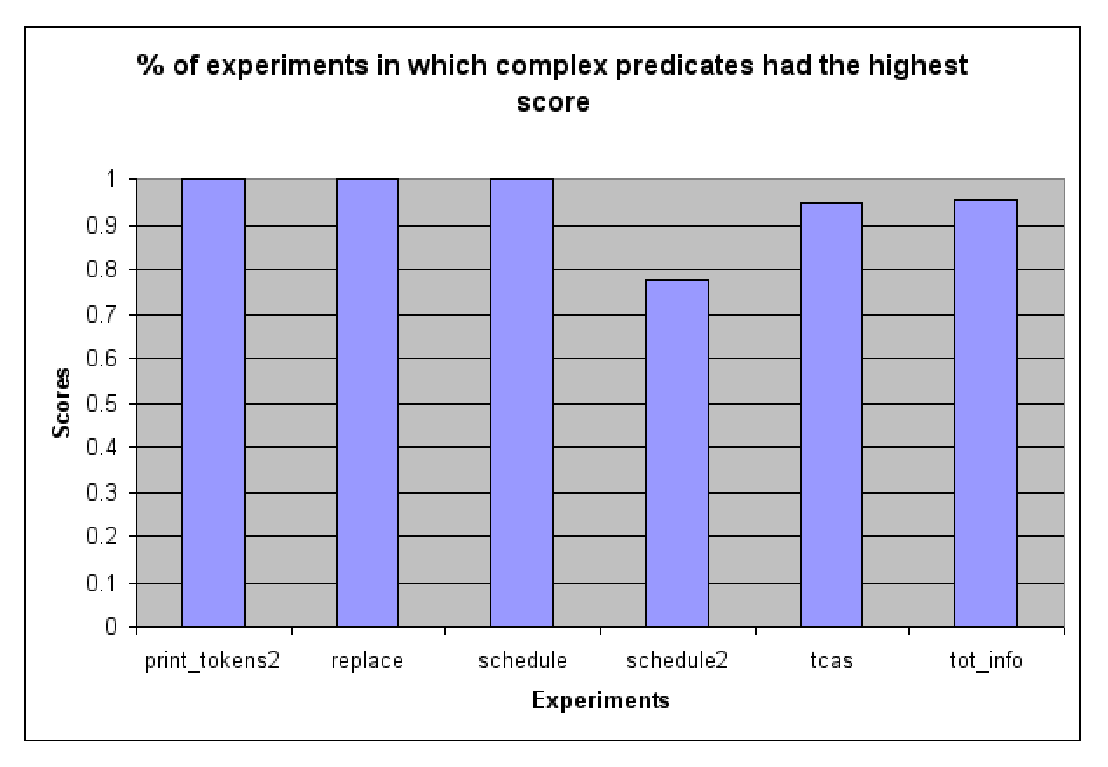
\includegraphics{charts/top-pred}
  \caption{Fraction of buggy application variants having a complex predicate as the top-scoring predictor}
  \label{fig-top-pred}
\end{figure}

\autoref{fig-top-pred} plots the percentage of variants within each program for which a complex predicate had the highest score among all predicates.  The value is 100\% for \texttt{print\_tokens2, replace} and \texttt{schedule} and is close to 100\% for the other programs.  The results shown in \autoref{fig-top-pred} combined with the case studies in \autoref{sec-qual} demonstrates the usefulness of complex predicates.

\subsection{Effectiveness of Pruning}

\begin{figure}
  \centering
  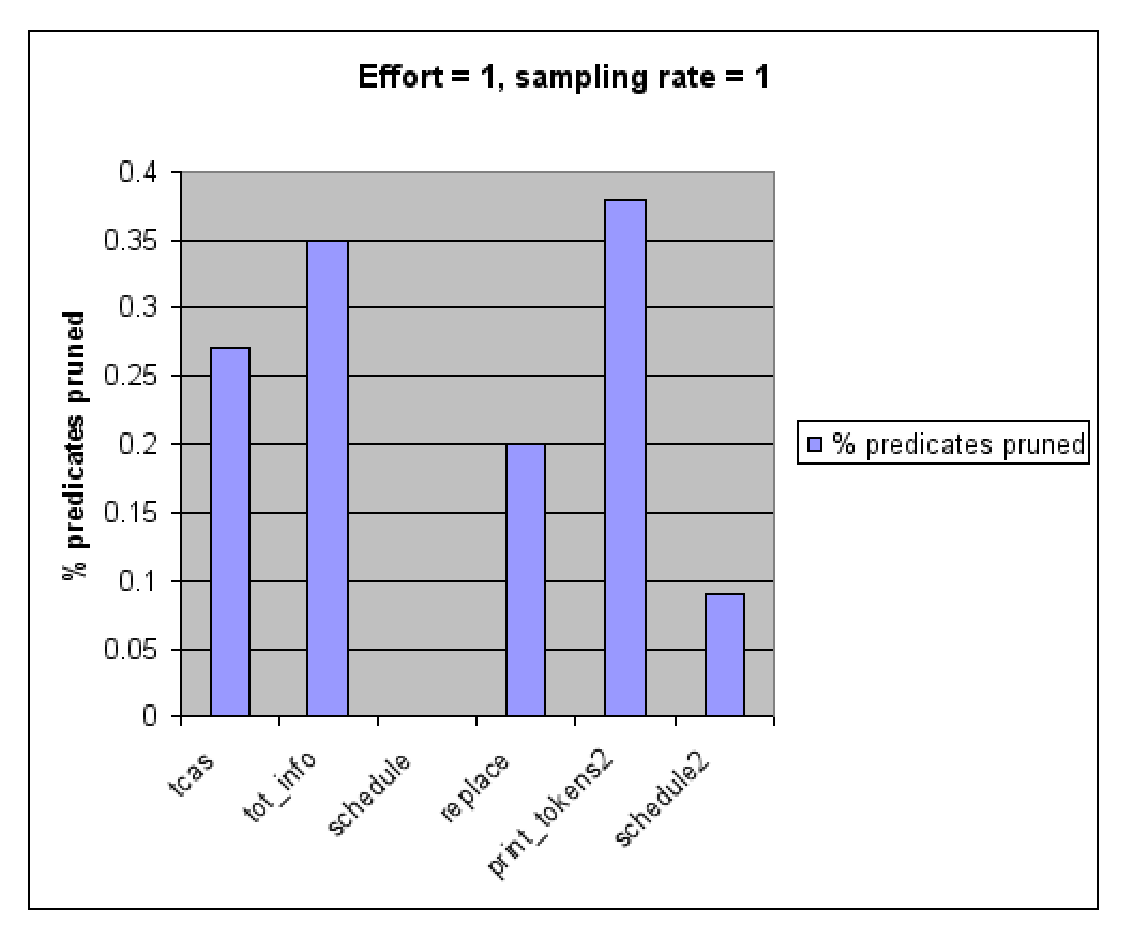
\includegraphics{charts/pruning}
  \caption{Avoiding computing exact scores by pruning complex predicates.  ``Overall'' summarizes the entire Siemens suite.}
  \label{fig-pruning}
\end{figure}

Even when restricted to binary conjunction and disjunction, complex predicates could substantially increase the analysis workload if na\"ively implemented.  \autoref{sec-metrics} suggests heuristics for pruning complex predicates which are unlikely to be useful or understandable to a programmer, while \autoref{sec-pruning} describes how to compute an upper bound on a predicate's score.  \autoref{fig-pruning} shows that these measures are highly effective in practice.  On average, 57\% of candidate complex predicates are discarded because the $\effort$ as defined in \autoref{def-effort} would require traversing more than 5\% of the application code.  A further 14\% of complex predicates are pruned because the upper bounds of their $\Importance$ scores, computed per \autoref{sec-pruning}, are lower than the scores of their constituent simple predicates.  Only 29\% of complex predicates remain.  Thus, exact scores need be computed for less than a third of the initial pool of complex predicates.

\subsection{Effect of Effort}

\begin{figure}
  \centering
  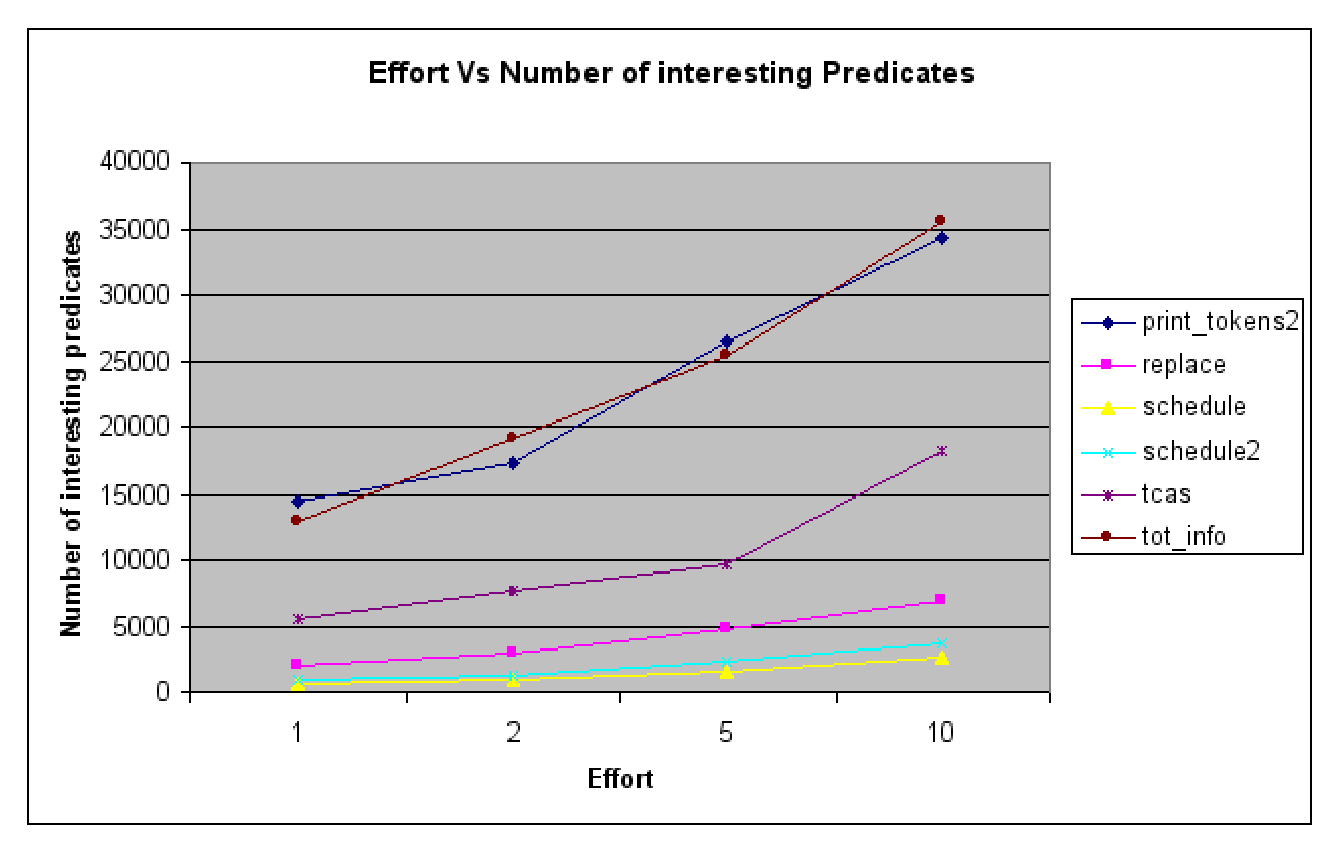
\includegraphics{charts/effort}
  \caption{Variation of number of interesting predicates with $\effort$}
  \label{fig-effort}
\end{figure}

\autoref{fig-effort} has one curve for each program showing how the number of interesting predicates (\autoref{dfn3}) varies at four different values - 1, 2, 5, 10 for $\effort$.  As expected, as $\effort$ increases more predicates are evaluated and so more interesting predicates are found.  This experiment serves as a sanity check for the implementation.

\subsection{Effect of Sampling Rate}
\label{sec-sampling}

\begin{figure*}
  \centering
  $\begin{array}{cc}
    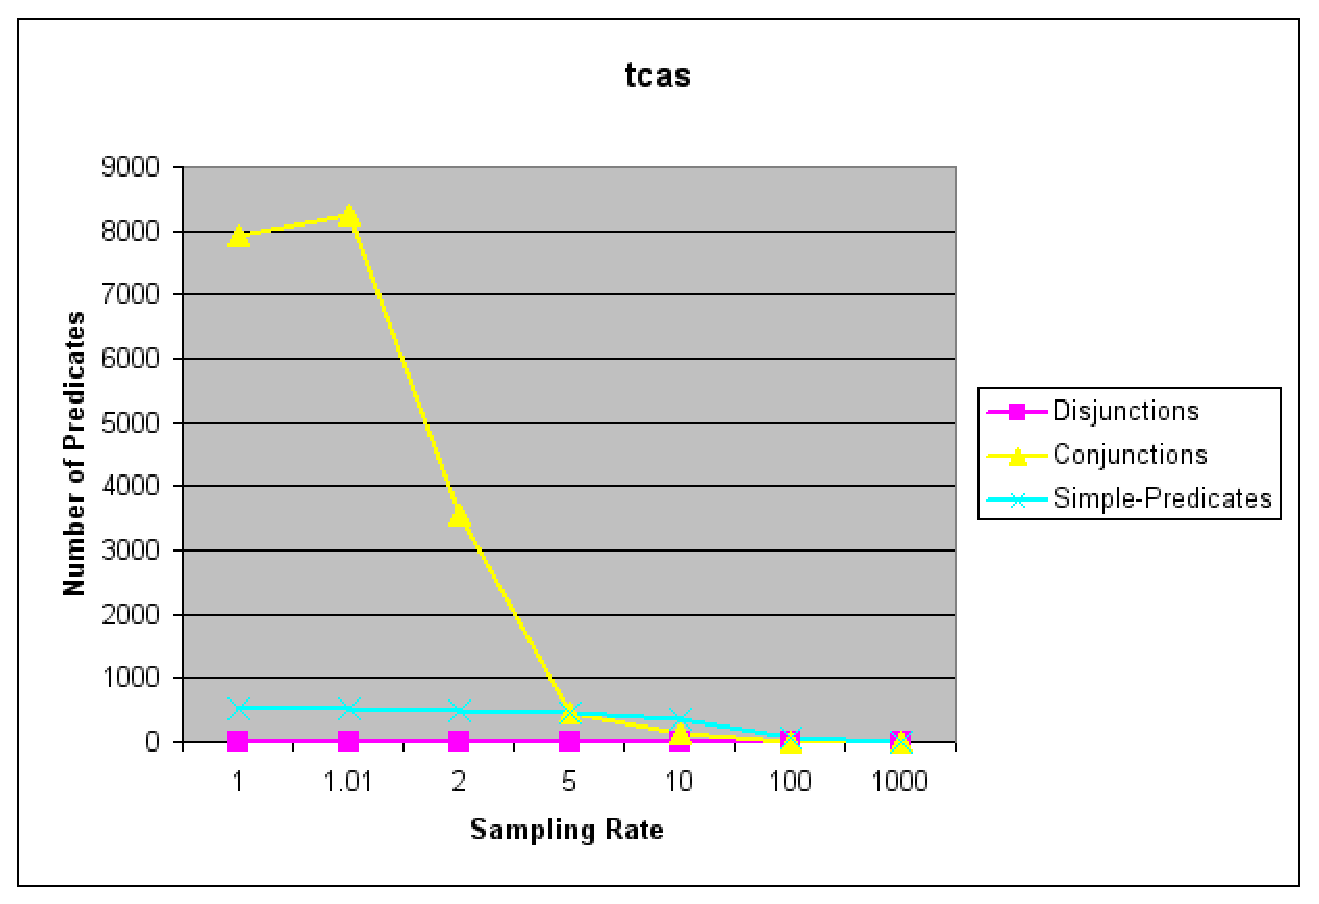
\includegraphics[width=\columnwidth]{charts/tcas} & 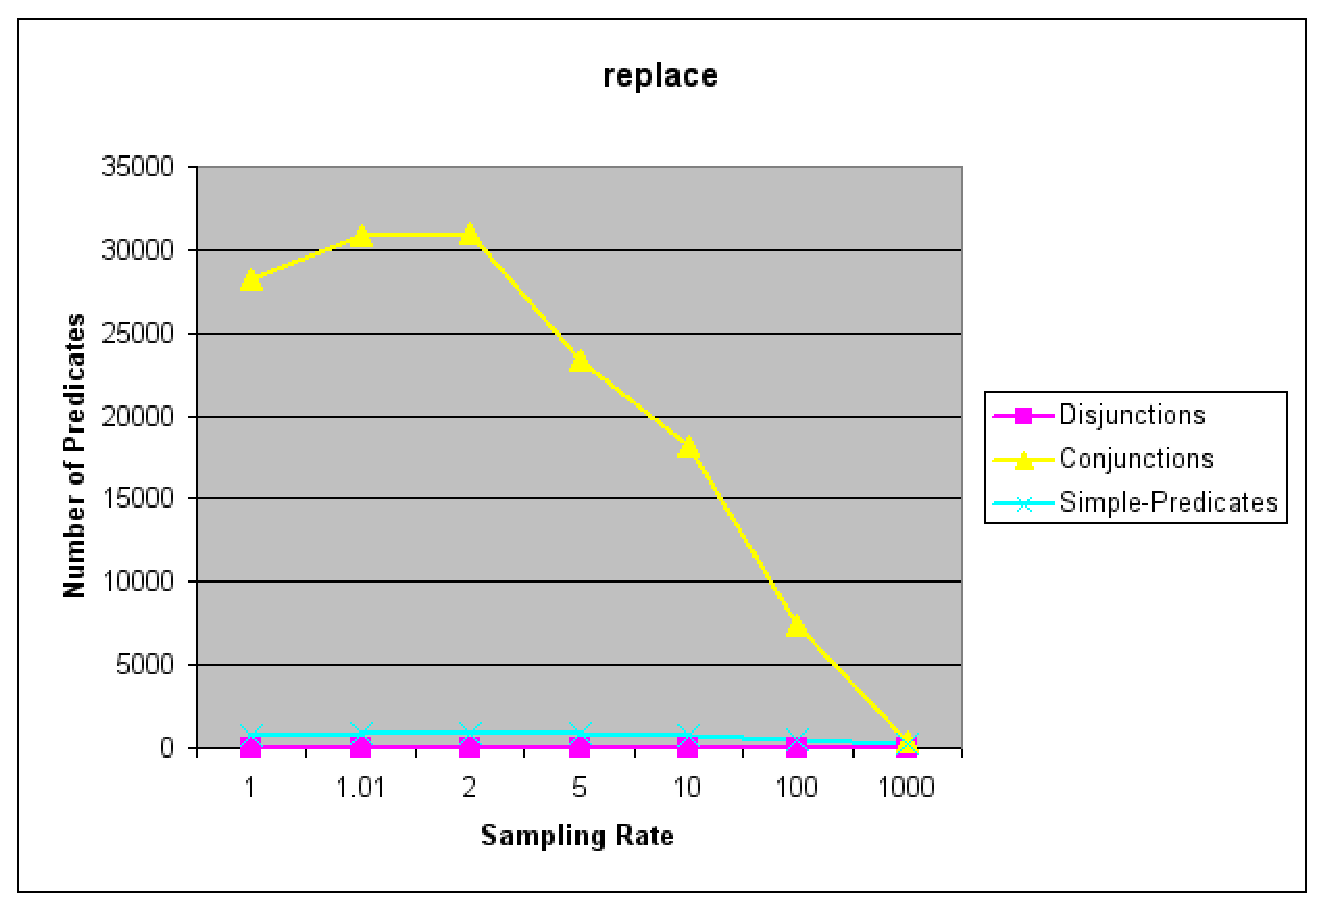
\includegraphics[width=\columnwidth]{charts/replace} \\
    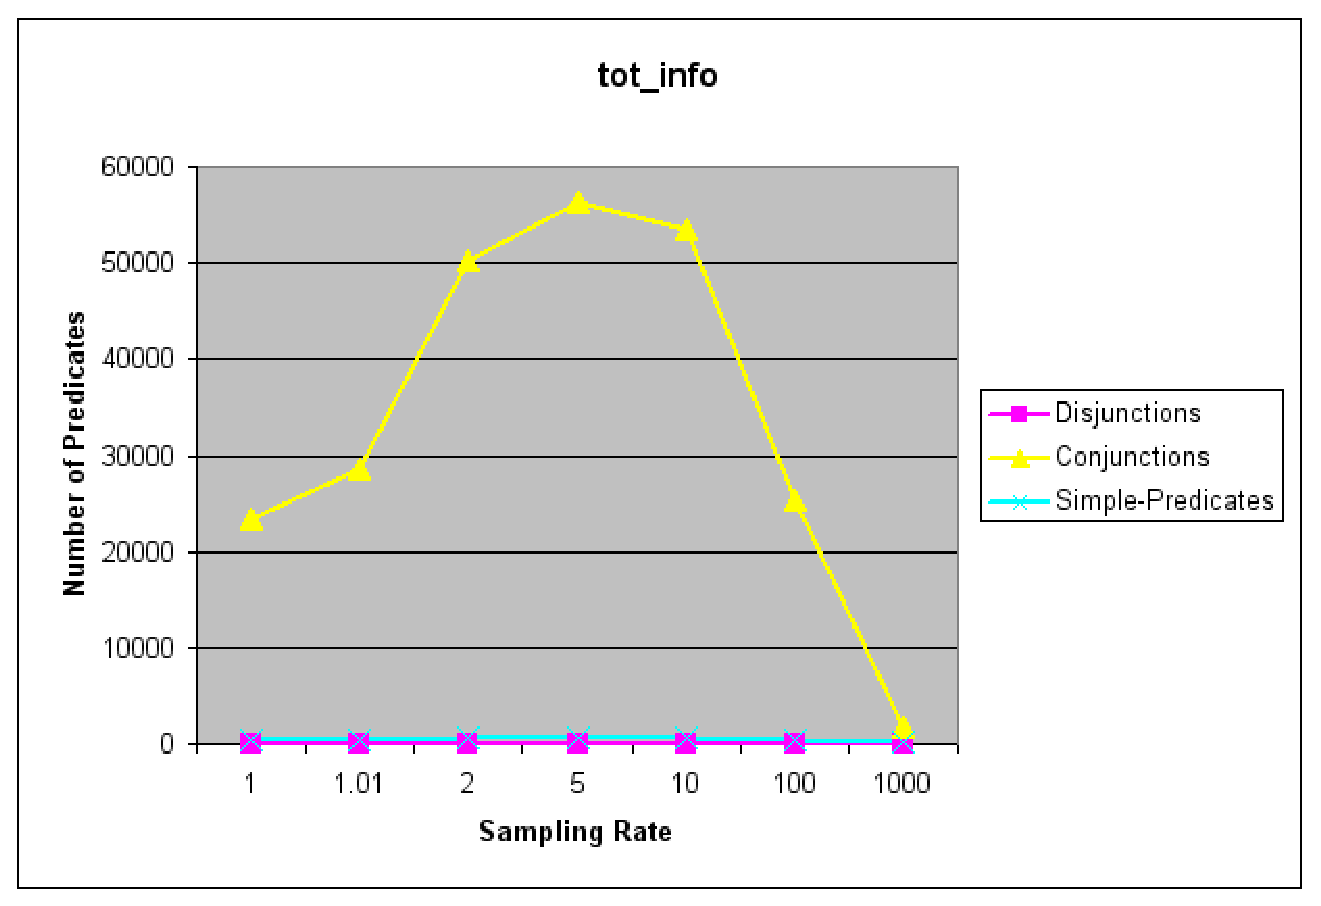
\includegraphics[width=\columnwidth]{charts/tot_info} & 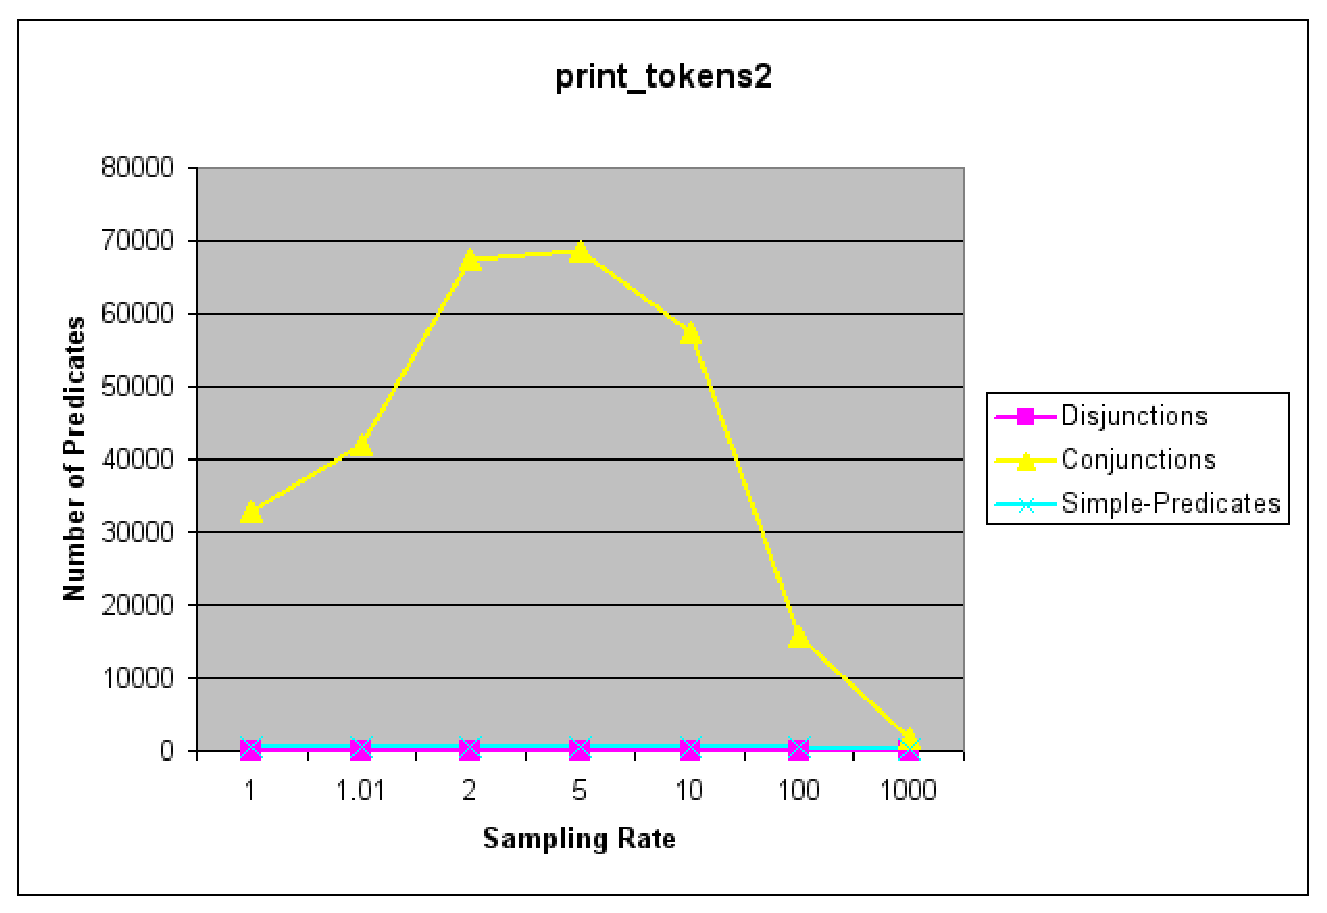
\includegraphics[width=\columnwidth]{charts/print_tokens2} \\
    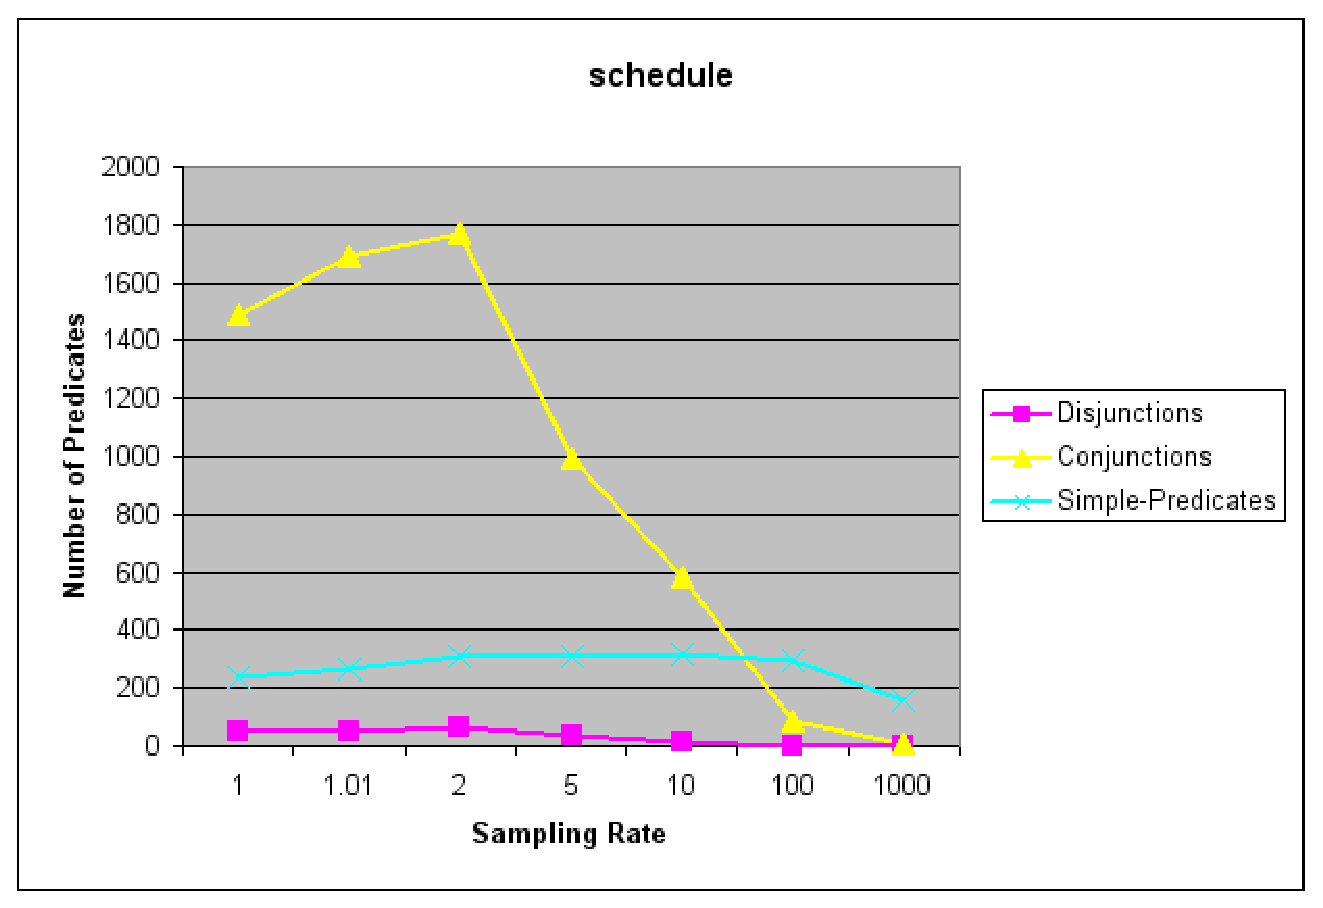
\includegraphics[width=\columnwidth]{charts/schedule} & 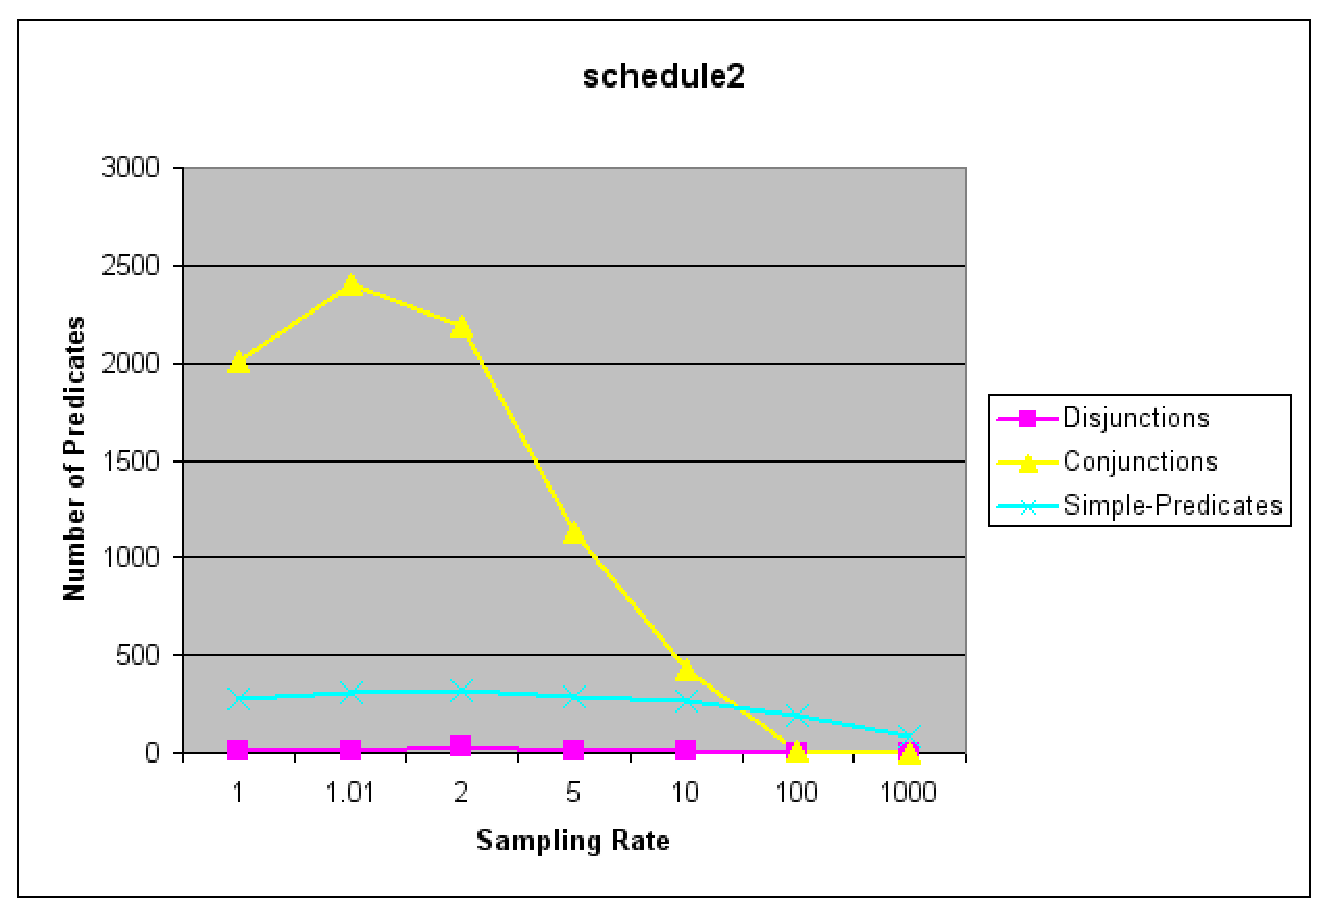
\includegraphics[width=\columnwidth]{charts/schedule2} \\
  \end{array}$
  \caption{Sampling Rate vs. Number of Interesting Predicates}
  \label{fig-sampling}
\end{figure*}

The dependence between sampling rate and the number of interesting predicates (both complex and simple) is plotted in \autoref{fig-sampling}.  \autoref{fig-sampling} has one chart per program with sampling rates in the $x-$axis and the average number of interesting conjunctions, disjunctions and simple predicates in the $y-$axis.  The number of interesting disjunctions is always very low (order of tens) compared to interesting conjunctions.  So the plot for interesting complex predicates closely follows the plot for conjunctions.  At sampling rates lower than \nicefrac{1}{10}, there is a sharp drop in the number of interesting conjunctions.  This is because the chance of observing both components of a conjunction within a single run falls with the square of the sampling rate.  Despite the sharp drop, the number of interesting conjunctions is still comparable to the number of interesting simple predicates even at \nicefrac{1}{1000} sampling.  This shows interesting complex predicates can still be found at sparse but realistic sampling rates.

A puzzling trend in \autoref{fig-sampling} is that the number of interesting conjunctions increases for a brief interval before dropping off.  This trend is consistent across all programs.  This can be due to two reasons:
\begin{enumerate}
\item Consider the $\Increase$ score (\autoref{eqn1}).  Sampling may be reducing the number of \emph{observed} runs in which a conjunction was true without affecting the \emph{true} runs.  This could happen because we do not collect sampled data directly but use scripts to downsample a data set collected with no sampling.  Because of binarization of counts, downsampling of a count from 100 to 99 does not affect the score whereas downsampling from 1 to 0 affects the score.
\item The script that does downsampling uses the standard pseudo random number generator.  Usually for experiments that use such random data, the values are averaged over multiple trials to get a confident estimate of the results.  We weren't able to conduct multiple trials because of time constraints.
\end{enumerate}

% -*- TeX-master: "master" -*-

\section{Related Work}
\label{sec-rw}
Daikon \cite{ErnstPGMPTX2006} detects invariants in a program by observing values computed by it over multiple program runs.  Invariants are predicates generated by using operators like sum, max, etc. to combine program variables and collection (e.g., array) objects.  Daikon is intended for many uses beyond bug isolation, and so it monitors a much larger set of predicates than CBI, which makes complex predicate generation more infeasible; despite this Dodoo et al. \cite{ErnstDRAFT} have successfully extended the work to generate implications from the simpler, measured predicates.  There are no known attempts to use Daikon under sparse sampling conditions.

SOBER \cite{1081753} is a statistical debugging tool similar to CBI.  Where CBI considers only whether a predicate was ever observed true during an execution, SOBER estimates the likelihood of it being true at any given evaluation.  When tested on the Siemens suite with full sampling this additional information resulted in better identification of bug predictors than traditional CBI analysis \cite{1081753}.  There are no known experiments using SOBER under sparse sampling conditions.  Since SOBER mimics CBI's structure, collecting data from deployed executions is possible, but SOBER analysis requires many more bits of data than CBI, increasing the burden on end users.

\subsection{Daikon and Complex Predicates}
\label{sec-daikon}
The system of generating complex predicates described in \cite{ErnstDRAFT} is very different from ours.  Dodoo et al. alternate clustering and invariant detection to find invariant implications over a set of program runs.  The initial clustering is performed using the k-means algorithm \cite{jain99data}, with program runs represented as normalized vectors of scalar variable values.  Since CBI represents run information as bit-vectors this technique can be applied essentially unchanged.

Daikon's implication generation extends the thoroughness of its invariant detection.  CBI's focus is detection of bug predictors, which under sparse sampling conditions can rarely be identified as invariant.  Additionally the fact that an implication exists is of questionable value in this project; the implication revealed in \autoref{sec-ccrypt} is an interesting and potentially useful side-effect of our analysis, but only because it involves identified bug predictors.  The approach described in this paper is better suited to the goals and analysis techniques of CBI.

DIDUCE \cite{581377} is inspired by Daikon, and detects invariant bits of numerical program values.  When operating in checking mode DIDUCE notifies the user the first time an inferred invariant is broken; the invariant is then relaxed to allow the new value.  Training mode functions the same way except that invariants are relaxed silently.  Both Daikon and CBI cleanly separate data collection and evaluation, whereas DIDUCE tightly couples the two.  Because of this coupling neither our approach to complex predicate generation nor Daikon's is easily applicable to DIDUCE's framework.

\subsection{SOBER and Complex Predicates}
CBI data is stored as a bit-vector for each program run, with each pair of bits (observed and true) representing a simple predicate.  SOBER data is a probability vector, with each value representing the estimated chance of a simple predicate being true when observed.  The similarity in collected data means that similar techniques for complex predicate generation are applicable.  The three-valued logic described in \autoref{sec-tvl} could be replaced with joint-probability when generating conjunctions; De Morgan's law can be applied to generate disjunctions.  Our usefulness metrics can be used on the resulting data.

Complex predicate generation removes a key advantage of SOBER - predicate scores result directly from the number of actual predicate evaluations.  Complex predicates generated by this technique are never truly evaluated, so their probability values would have little connection to actual program execution.  Whether this would affect their usefulness is unknown.

\section{Conclusion}
\label{sec-conc}
We have demonstrated that complex predicates are useful predictors of bugs.  Our experiments show qualitative and quantitative evidence that complex predicates can improve the current statistical analysis used by CBI.  We describe two optimizations that make the task of computing complex predicates feasible.  First is a numeric estimate on the upper bound of the score of a complex predicate.  The second is a metric that quantifies the usefulness of a complex predicate.  Even after these, the computational complexity is still high and requires further optimizations.  The metrics described in section ~\ref{sec-metrics} help reduce the number of spurious predicates.  But the metrics are not perfect as good bug predictors are still swamped by less useful ones.  The algorithm described in ~\ref{Zheng:2006:SDSIMB} may solve this problem as it was designed with the goal of handling multiple predictors for the same bug.
% -*- TeX-master: "report" -*-

\section*{Acknowledgments}

We would like to thank Anne Mulhern for her insightful comments on an earlier draft of this paper.


\bibliographystyle{abbrv}
\bibliography{local}

\end{document}
